\section{Валидация результатов}

\indent
\indent
Эта глава посвящена процедуре валидации предлагаемых 
хэштегов с привлечением пользователей социальной сети 
\textit{Одноклассники}\footnote{ok.ru/}.


\begin{figure}
    \begin{center}
   	    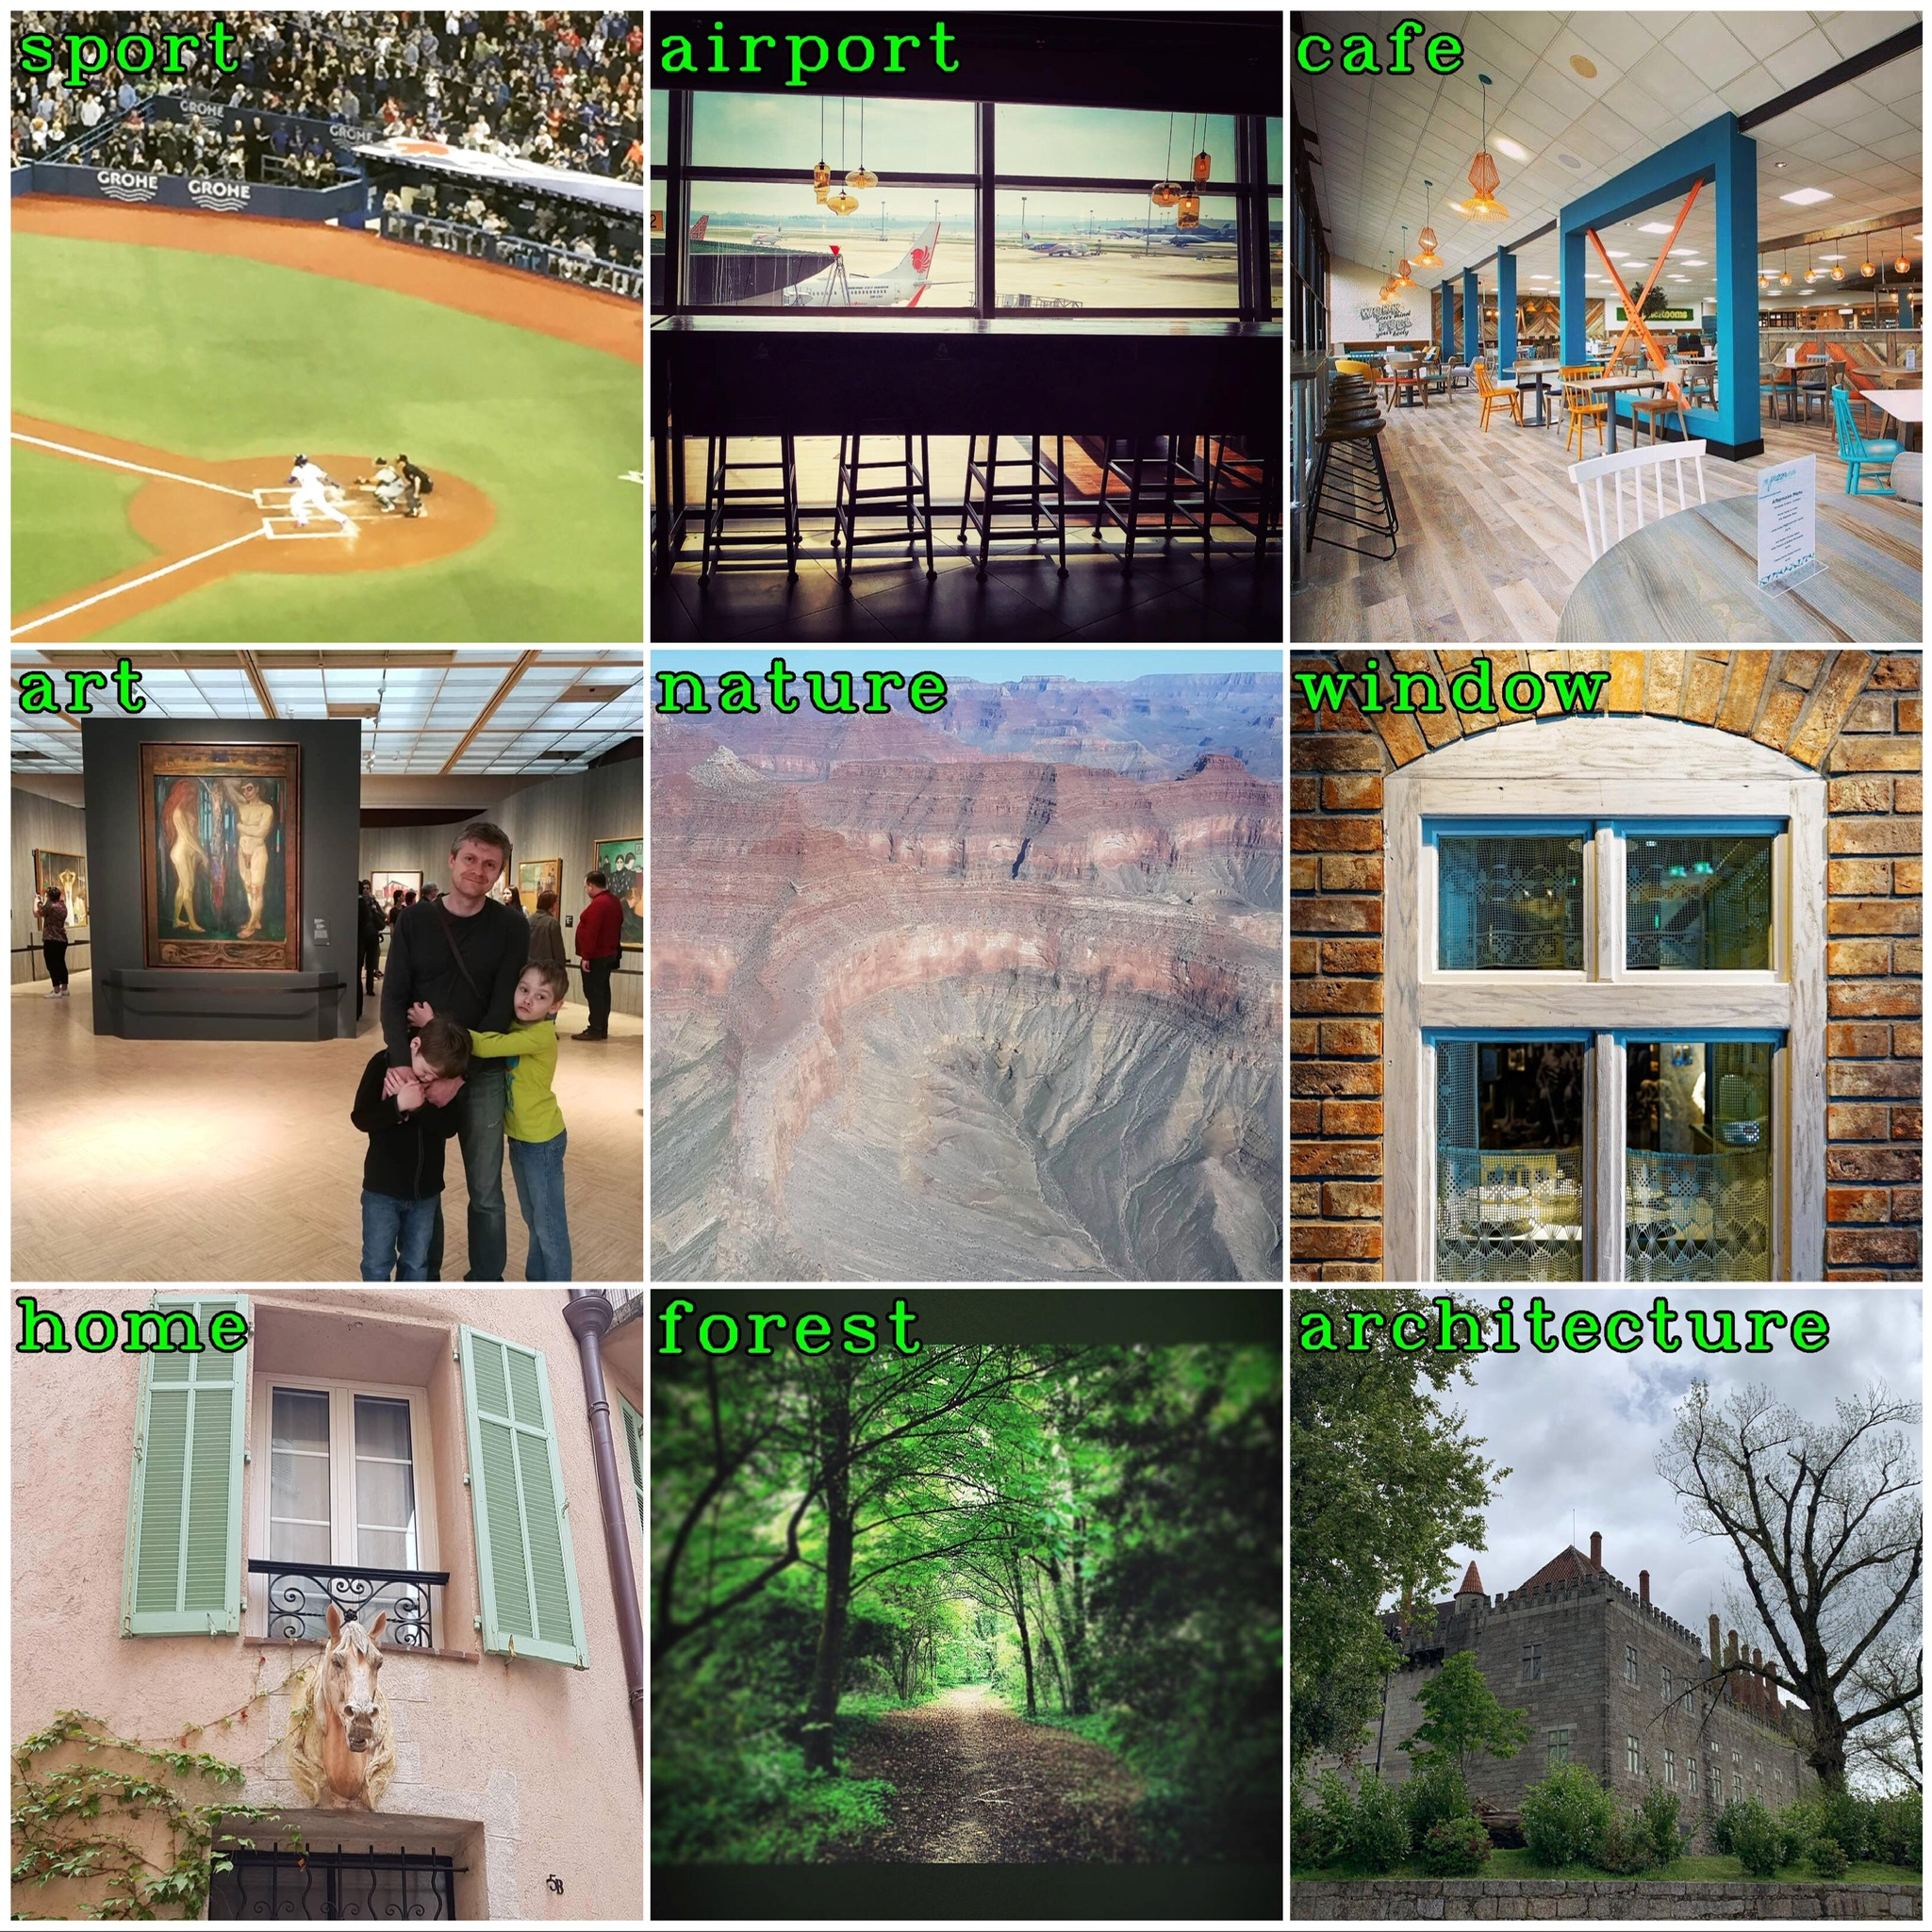
\includegraphics[width=0.9\linewidth]{insta_predict}
   	\end{center}
   	\caption{Примеры, для которых предсказанные
   	 \textit{(predicted)} и истинные \textit{(ground truth)} классы совпадают.}
   	\label{tikzpicture: correct_predict}
\end{figure}



todo
1. скачиваю изображения из insta
2. предсказываю для них тег моделью
3. отдаю пользователям, которые либо считают предсказанный 
тег подходящим, либо нет.
4. привожу долю тегов, которые пользователи посчитали подходящими.